
\begin{figure}[htbp]
    \begin{subfigure}[]{0.5\textwidth}
    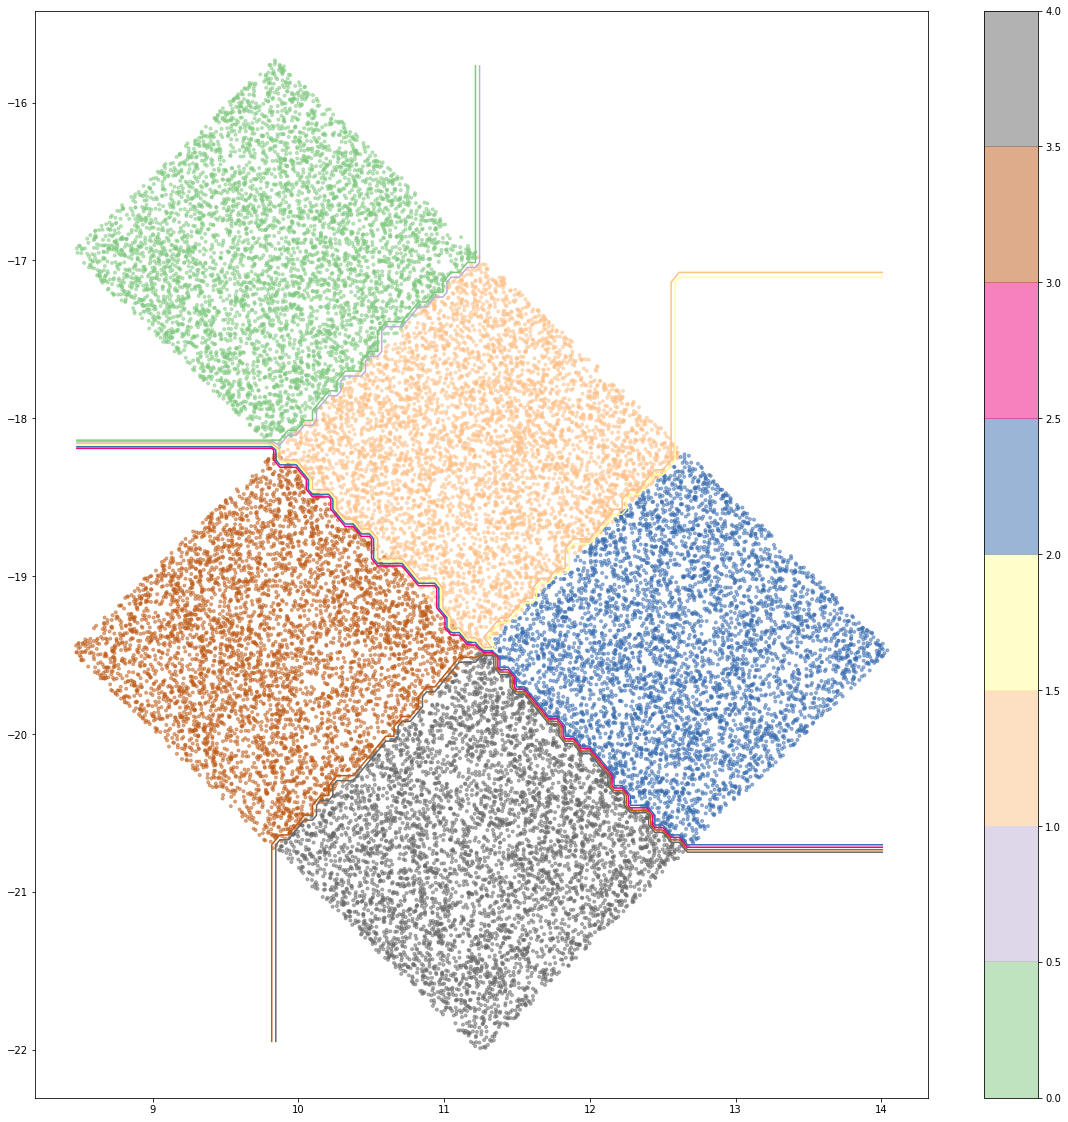
\includegraphics[width=\textwidth]{images/A2_prototypes/tu_multifile_tree.png}
    \caption{Without overlap}\label{subfig:tu_multifile}
    \end{subfigure}
    \hfill
    \begin{subfigure}[]{0.5\textwidth}
    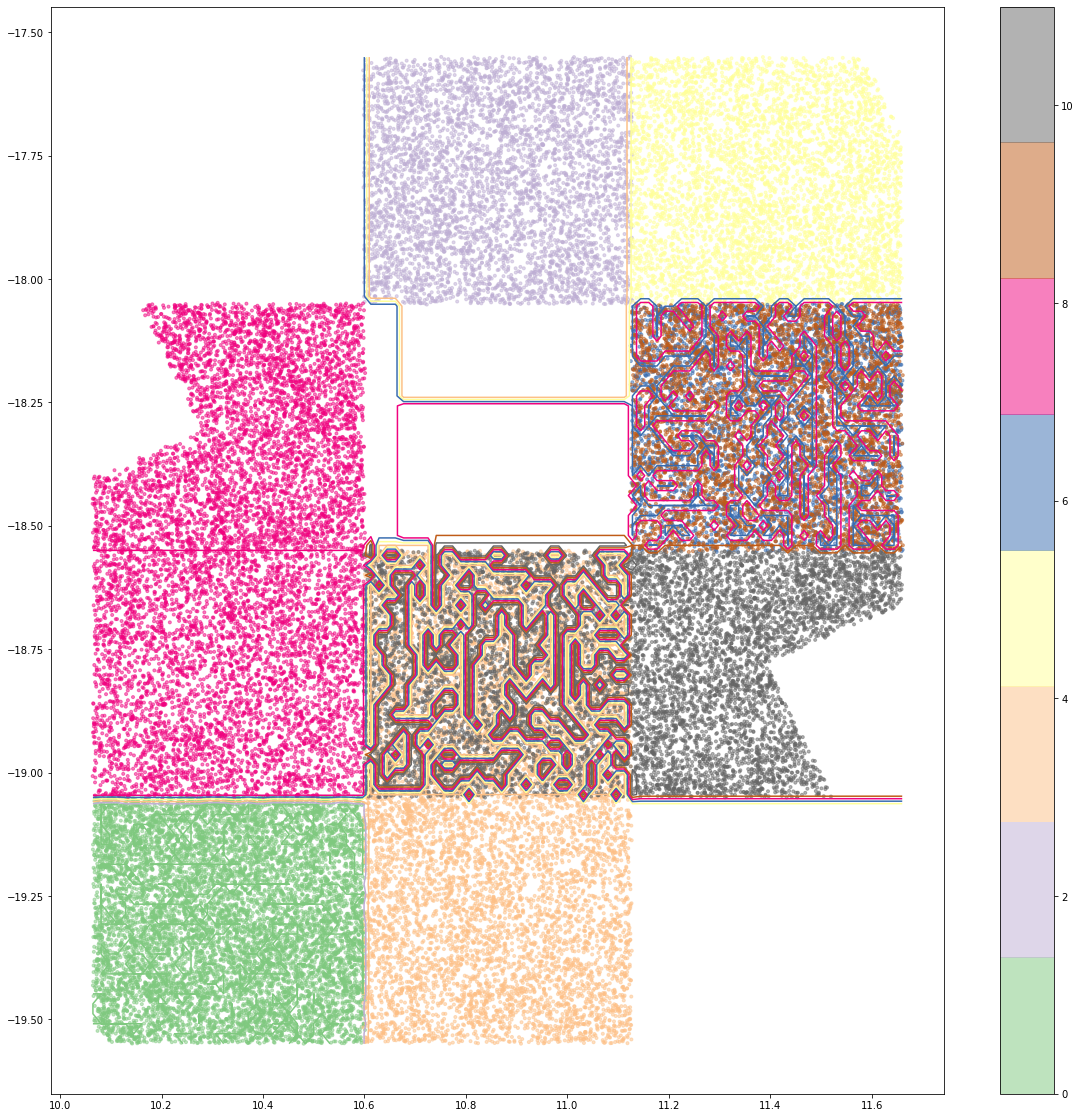
\includegraphics[width=\textwidth]{images/A2_prototypes/mer_multifile_tree.png}
    \caption{With overlap}\label{subfig:mer_multifile}
    \end{subfigure}
    \caption{
        Data-sets distributed multiple files based on two spatial coordinates.
        Each color corresponds to a single file.
    }
    \label{fig:tree_cat_cut}
\end{figure}

\begin{figure}[htbp]
    \centering
    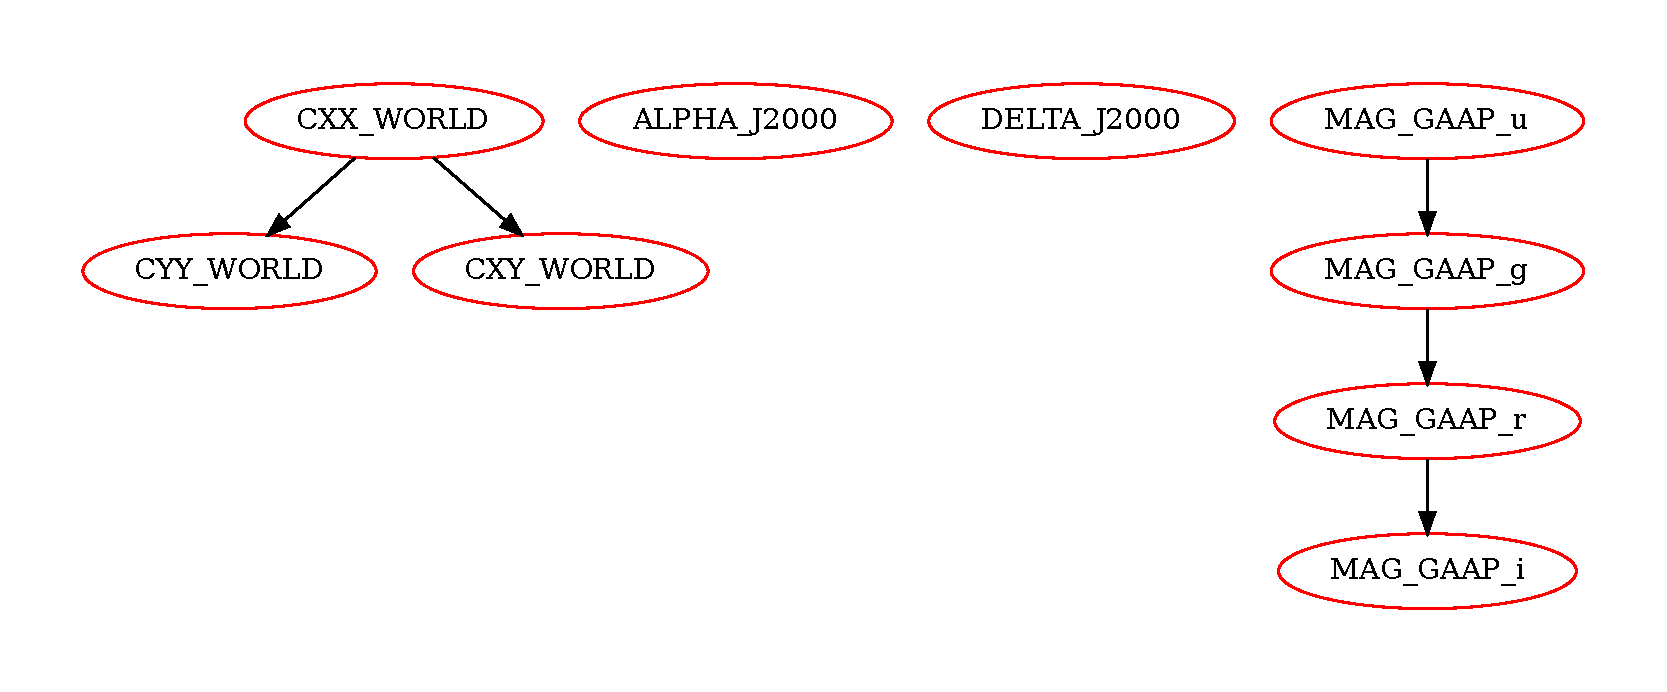
\includegraphics[width=\linewidth]{images/A2_prototypes/png_kids.pdf}
    \caption{Caption}
    \label{fig:prototype_png_kids}
\end{figure}

\begin{figure}[htbp]
    \centering
    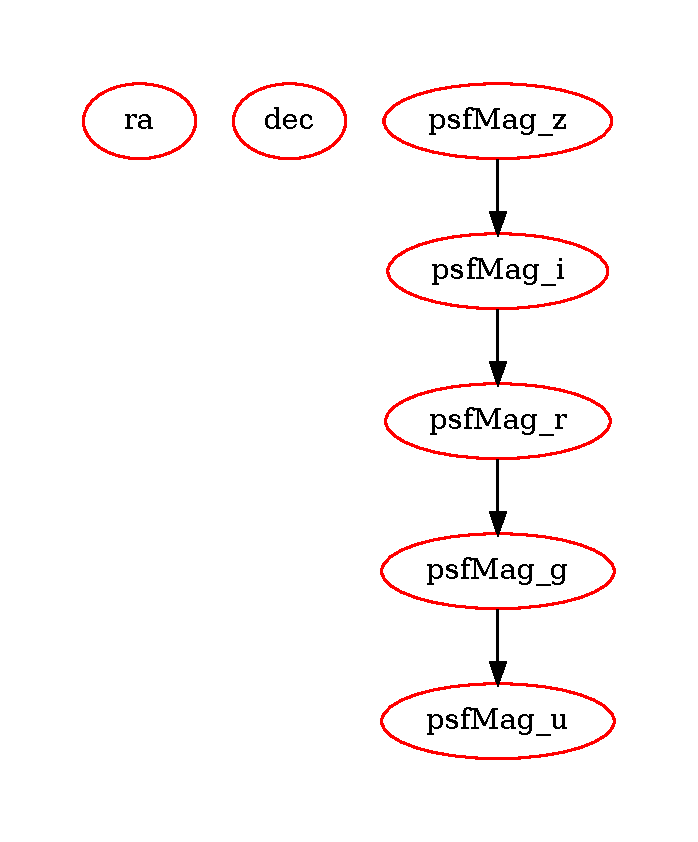
\includegraphics[width=\linewidth]{images/A2_prototypes/png_sdss.pdf}
    \caption{Caption}
    \label{fig:prototype_png_sdss}
\end{figure}